\subsubsection{Schritt 3: Erzeugen von ben�tigten Komponenten}\label{sem_eval_step3}
Eine ben�tigte Komponente besteht aus einer Kombination von Methoden-Konvertierungsvarianten, wobei f�r jede erwartete Methode genau eine Methoden-Konvertierungsvariante innerhalb der ben�tigten Komponente existiert.\\\\
F�r die Ermittlung der Kombinationen von Methoden-Konvertierungsvarianten wird eine Kombination von Typ-Konvertierungsvarianten aus der Ergebnismenge des zweiten Schrittes im aktuellen Durchlauf  selektiert. Die daraus erzeugten Methoden-Konvertierungsvarianten werden hinsichtlich der Methoden aus dem erwarteten Interface miteinander kombiniert.\\\\
F�r die erste Kombination von Typ-Konvertierungsvarianten, die \abbref{tkv_alv_alu_1} zu entnehmen ist ($TKV_{AIv}$),  k�nnen folgende Kombinationen von Methoden-Konvertierungsvarianten erzeugt werden (siehe \abbref{comb_mkv_alv_1}).
\myBigFigure{comb_mkv_alv_1}{Kombinationen von Methoden-Konvertierungsvarianten AIv}{comb_mkv_alv_1}
\noindent
Analog dazu wird f�r die zweite Kombination von Typ-Konvertierungsvarianten, die \abbref{tkv_alv_alu_1} zu entnehmen ist ($TKV_{AIu}$), folgende Kombination von Methoden-Konvertierungsvarianten erzeugt (siehe \abbref{comb_mkv_alu_1}).\\\\
Ausgehend von der Kombination von Typ-Konvertierungsvarianten aus \abbref{comb_tkv_alv_alu_1} ($TKV_{AIu+AIv}$), sind in \abbref{comb_mkv_alu_alv} die daraus resultieren Methoden-Konvertierungsvarianten dargestellt.Zu beachten ist, dass die ersten vier Kombinationen bereits im vorherigen Durchlauf erzeugt wurden (siehe \abbref{comb_mkv_alv_1}) und dementsprechend auch getestet wurden.



\begin{figure}[H]
\begin{minipage}[b]{.38\linewidth}
  \centering
  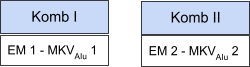
\includegraphics[width=.6\linewidth]{comb_mkv_alu_1}
  \caption{Kombinationen von Methoden-Konvertierungsvarianten AIu}
  \label{abb:comb_mkv_alu_1}

\end{minipage}%
\hspace{.04\linewidth}% Abstand zwischen Bilder
\begin{minipage}[b]{.58\linewidth}


  \centering
  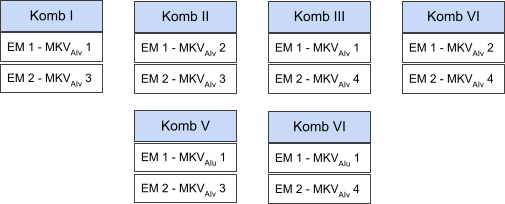
\includegraphics[width=\linewidth]{comb_mkv_alu_alv}
  \caption{Kombinationen von Methoden-Konvertierungsvarianten AIu+AIv}
  \label{abb:comb_mkv_alu_alv}

\end{minipage}
\end{figure}
\noindent
Im Allgemeinen l�sst sich sagen, dass die Anzahl der Kombinationen von Methoden-Konvertierungsvarianten von der Anzahl der Methoden im erwarteten Interface ($|EM|$) und der Anzahl von Methoden-Konvertierungsvarianten ($|MKV|$), die aus der selektierten Kombination von Typ-Konvertierungsvarianten erzeugt werden k�nnen. Da aus einer Kombination von Methoden-Konvertierungsvarianten jeweils eine ben�tigte Komponente erzeugt werden kann, gilt f�r die Anzahl der ben�tigten Komponenten ($|Komb_{ben}|$) dasselbe. Im schlimmsten Fall berechnet sich die Anzahl der ben�tigten Komponenten wie folgt:
\begin{align*}
|Komb_{ben}| = |Komb_{MKV}| = \frac{|MKV|!}{(|MVK| - |EM|)!*|EM|!}
\end{align*}

